\scanpage{47}
% E: text|upper left, l|Loi de symétrie
l) Loi de symétrie autour d'un côté exceptionnel (\unsure{y compris un côté fermé}), et structure locale autour d'une composante exceptionnelle de \(K\)

% E: drawing|left centre, long coloured configuration|six green transversals and red curves
\figure{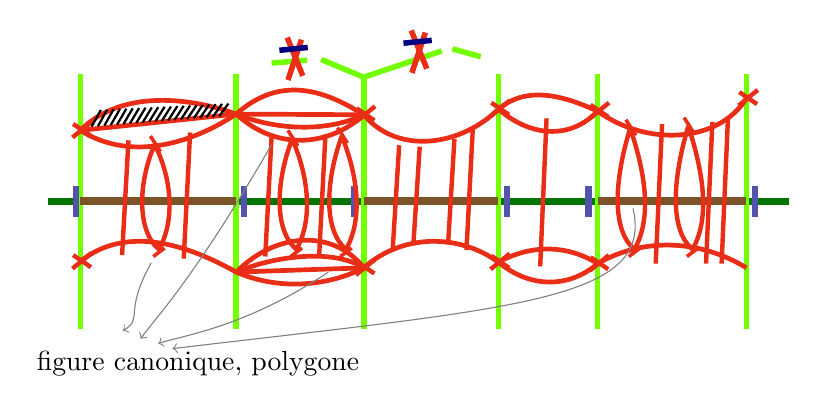
\begin{tikzpicture}[x=.9cm,y=.9cm]
\draw[green!45!black,line width=2.4pt](-.45,0)--(10,0);
\foreach \x in {0,2.2,4,5.9,7.3,9.4}{\draw[green!55!yellow,line width=2pt](\x,-1.8)--(\x,1.8);}
\foreach \a/\b in {0/2.2,4/5.9,7.3/9.4}{\draw[brown!65!black,line width=3pt](\a,0)--(\b,0);}
\foreach \x in {-.06,2.31,3.87,6.02,7.17,9.52}{\draw[blue!35!gray,line width=2.3pt](\x,-.22)--(\x,.22);}
\draw[red!65!brown,line width=1.7pt](0,1)..controls(.6,1.6)and(1.6,1.45)..(2.2,1.23)..controls(2.8,1.76)and(3.4,1.6)..(4,1.22)..controls(4.5,.63)and(5.4,.8)..(5.9,1.3)..controls(6.3,1.63)and(6.8,1.5)..(7.3,1.27)..controls(8,.77)and(9,.82)..(9.4,1.45);
\draw[red!65!brown,line width=1.7pt](0,1)..controls(.7,.56)and(1.55,.8)..(2.2,1.23)..controls(2.8,.68)and(3.55,.8)..(4,1.22);
\draw[red!65!brown,line width=1.7pt](0,1)--(2.2,1.23)--(4,1.22);
\draw[red!65!brown,line width=1.7pt](2.2,1.23)..controls(2.8,.99)and(3.5,.98)..(4,1.22);
\draw[red!65!brown,line width=1.7pt](5.9,1.3)..controls(6.4,.87)and(6.95,.9)..(7.3,1.27);
\draw[red!65!brown,line width=1.7pt](0,-.85)..controls(.6,-.37)and(1.4,-.55)..(2.2,-1.0)..controls(2.8,-.4)and(3.6,-.42)..(4,-.94)..controls(4.55,-.45)and(5.35,-.46)..(5.9,-.86)..controls(6.4,-.59)and(6.9,-.63)..(7.3,-.88)..controls(8,-.48)and(8.8,-.57)..(9.4,-.94);
\draw[red!65!brown,line width=1.7pt](2.2,-1)..controls(2.9,-1.3)and(3.6,-1.15)..(4,-.94);
\draw[red!65!brown,line width=1.7pt](2.2,-1)..controls(2.8,-.75)and(3.6,-.68)..(4,-.94);
\draw[red!65!brown,line width=1.7pt](2.2,-1)--(4,-.94);
\draw[red!65!brown,line width=1.7pt](5.9,-.86)..controls(6.4,-1.27)and(6.95,-1.19)..(7.3,-.88);
\foreach \x/\u/\v in {.68/.86/-.76,1.55/.97/-.81,2.7/.92/-.78,3.46/.94/-.78,4.5/.79/-.66,4.79/.77/-.62,5.28/.88/-.61,5.54/1.04/-.69,6.58/1.17/-.92,8.21/1.09/-.88,8.92/1.12/-.88,9.14/1.18/-.88}{\draw[red!65!brown,line width=1.6pt](\x,\u)--(\x-.09,\v);}
\foreach \x/\y in {1.05/.8,2.99/.88,3.69/.92,7.76/1.03,8.58/1.06}{\draw[red!65!brown,line width=1.6pt](\x,\y)..controls(\x-.24,.25)and(\x-.25,-.42)..(\x+.06,-.68)..controls(\x+.3,-.25)and(\x+.23,.35)..(\x,\y);\draw[red!65!brown,line width=1.3pt](\x-.06,\y+.12)--(\x+.08,\y-.1);\draw[red!65!brown,line width=1.3pt](\x-.02,-.78)--(\x+.14,-.66);}
\foreach \x/\y in {0/1,0/-.85,4/1.22,4/-.94,5.9/1.3,5.9/-.86,7.3/1.27,7.3/-.88,9.4/1.45}{\draw[red!65!brown,line width=1.6pt](\x-.11,\y-.1)--(\x+.16,\y+.12);\draw[red!65!brown,line width=1.6pt](\x-.1,\y+.09)--(\x+.15,\y-.08);}
\foreach \x in {.16,.25,.34,.43,.52,.61,.7,.79,.88,.97,1.06,1.15,1.24,1.33,1.42,1.51,1.60,1.69,1.78,1.87,1.96}{\draw[black,line width=.8pt](\x,1.04+\x*.08)--(\x+.13,1.28+\x*.05);}
\draw[green!55!yellow,line width=2pt](2.7,1.95)--(3.2,1.99);\draw[green!55!yellow,line width=2pt](3.4,2)--(4,1.75)--(5.1,2.12);\draw[green!55!yellow,line width=2pt](5.25,2.15)--(5.65,2.04);
\foreach \x/\y in {3/2.07,4.75/2.17}{\draw[red!65!brown,line width=2pt](\x-.08,\y+.24)--(\x+.14,\y-.3);\draw[red!65!brown,line width=2pt](\x+.12,\y+.21)--(\x-.07,\y-.36);\draw[blue!50!black,line width=2pt](\x-.19,\y+.06)--(\x+.21,\y+.1);}
\draw[gray,->](1,-.87)..controls(.6,-1.6)and(.9,-1.64)..(.6,-1.83);
\draw[gray,->](2.7,.8)..controls(1.6,-1.1)and(1.1,-1.6)..(.85,-1.94);
\draw[gray,->](3.5,-1)..controls(2.3,-1.8)and(1.4,-1.9)..(1.1,-2.01);
\draw[gray,->](7.8,-.1)..controls(8.1,-1.4)and(6.2,-1.5)..(1.3,-2.08);
\node[below right]at(-.75,-1.98){figure \unsure{canonique}, \deleted{\unsure{polygone}}};
\end{tikzpicture}}
\margin{\deleted{\unsure{voir}} i) j) ---}

% E: text|left below drawing, m|Indexation des sections
m) Indexation des sections de \(L\) sur les faces de \((X,K)\) \deleted{à l'aide de} par \(\widetilde I\), et passage d'une indexation à l'indexation de la face adjacente.

% E: text|lower left, n|Reconstitution de
n) Reconstitution de \deleted{\(\unsure{\xi}\)} \(\underline\Sigma\) (via \(\widetilde I\) ---) à l'aide de \(K\), et des constantes numériques associés à \(K\) (indices des sommets de \(K\)\inserted{\(\unsure{i(s)}\in\unsure{\frac12\mathbb Z|\frac12\mathbf Z}\) et \(\nu(s)\in\mathbb N\)}\inserted{\unsure{noté}}, \(\nu(a)\) des arêtes de \(K\)\deleted{\unsure{antiques}} \deleted{\(\unsure{\varphi}\)} (distinguons le cas des côtés ord\unsure{res} et des côtés exceptionnels.) Cf. aussi

\margin{\uline{NB} l'indice de chaque côté exceptionnel stable est \(\unsure{=|\geq}n-(\nu_s-1)-(\nu_t-1)\)\deleted{\(\unsure{\leq n}\)} et les instables \(\unsure{=|\geq}n-\nu\), où \(\nu\) est la multiplicité du sommet --- et la figure ci-contre est correcte ! On voit que l'indice des arêtes exceptionnelles résulte des autres données numériques.}

% E: text|right upper, NB|Il y a évidemment
\uline{NB} Il y a évidemment une loi de symétrie autour d'un côté ordinaire, pour ce qui est de la configuration induite par \(L\) sur les 2 faces adjacentes, au voisinage de l'arête en question. Peut-être $=$ \unsure{ceci est induit} : Considérer le couple \((X,K\cup L)\), et ``le voisinage ``tubulaire'' \unsure{standart}'' \(\overline T\) (\unsure{réunion d'``étoiles''}), du \deleted{\(K\) des côtés}\inserted{sous-complexe \(K\) de} \(K\cup L\) des arêtes \unsure{criti.} \deleted{\unsure{ordinaires}}. Alors pour toute arête \(a\) de \(K\), posant

% E: drawing|right centre, local crossing and curved edges|green T and red configuration
\figure{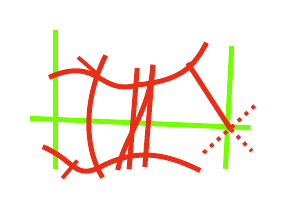
\begin{tikzpicture}[scale=.8]
\draw[green!55!yellow,line width=1.8pt](-.4,0)--(3.1,-.15);\draw[green!55!yellow,line width=1.8pt](0,-.8)--(0,1.4);\draw[green!55!yellow,line width=1.8pt](2.7,-.8)--(2.8,1.15);
\draw[red!65!brown,line width=1.8pt](-.1,.65)..controls(.7,1)and(.7,.35)..(1.3,.53)..controls(2,.6)and(2.2,.82)..(2.4,1.2);
\draw[red!65!brown,line width=1.8pt](-.2,-.45)..controls(.3,-.66)and(.3,-.97)..(.7,-.78)..controls(1.3,-.45)and(1.8,-.58)..(2.3,-.83);
\draw[red!65!brown,line width=1.8pt](.8,1)..controls(.4,.2)and(.5,-.55)..(.75,-.94);
\draw[red!65!brown,line width=1.8pt](1.3,.8)--(1.17,-.81);\draw[red!65!brown,line width=1.8pt](1.55,.85)--(1.42,-.77);
\draw[red!65!brown,line width=1.8pt](1.55,.85)..controls(1.5,.1)and(1.1,-.28)..(.99,-.82);
\draw[red!65!brown,line width=1.8pt](2.1,.88)--(2.78,-.17);\draw[red!65!brown,line width=1.4pt,dotted](2.35,-.55)--(3.22,.25);\draw[red!65!brown,line width=1.4pt,dotted](2.78,-.17)--(3.12,-.52);
\draw[red!65!brown,line width=1.4pt](.36,.97)--(.67,.7);\draw[red!65!brown,line width=1.4pt](.11,-.95)--(.35,-.67);
\end{tikzpicture}}

% E: display|right lower, definition T_a|T_a definition
\[
\overline T_a\overset{\mathrm{def}}=(F'\cup F'')\cap\overline T,
\]
% E: text|right lower, after T_a|F' F'' sont
\(F',F''\) sont les deux faces de \((\unsure{X},K)\) incidentes à \(a\); on a une involution \deleted{\(\unsure{\varphi}\)} \(\sigma_a\) de \(\unsure{a|\overline T_a}\), \unsure{ayant} \(a\) comme lieu de pts fixes, et qui \unsure{respecte} la structure \unsure{cellulaire} induite par \((X,K\cup L,\underline{\unsure{D}}\) \unsure{plus}, \deleted{\unsure{si \(a\) et \(b\)}} deux incidents au $=$ sommet \(s\), alors \(\sigma_a|\overline T_a\cap\overline T_b\) et \(\sigma_b|\overline T_a\cap\overline T_b\) \unsure{commutent les uns aux autres}.
\mspage{46}
